\documentclass[aspectratio=169,11pt]{beamer}
\usepackage{beamertemplate}
\usepackage{graphicx}
\usepackage{booktabs}
\usepackage{url}
\usepackage{textcomp}
\usepackage{eurosym}
\usepackage[normalem]{ulem}
\usepackage{ragged2e}
\usepackage{etoolbox}
\apptocmd{\itemize}{\justifying}{}{}
\AtBeginEnvironment{frame}{\justifying}

% Formato uniforme para comandos, ficheros y rutas
\newcommand{\cmd}[1]{\texttt{#1}}
% Rótulo uniforme para el encabezado de contenido dentro de un frame
\newcommand{\lead}[1]{{\bfseries #1}\par\medskip}

% Repite el índice al empezar cada sección, resaltando la que comienza
\setbeamertemplate{section in toc shaded}[default][30]
\AtBeginSection[]{%
  \begin{frame}{Índice}
  \footnotesize
  \tableofcontents[currentsection]
  \end{frame}
}

\title[SSI -- Tema 3.1]{Ataques a las credenciales}
\subtitle{Seguridad en Sistemas Informáticos --- Tema 3.1}
\author{José Luis Martínez}
\institute{Universidad de Castilla-La Mancha}
\date{Curso 2026/27}

% --- build reproducible / metadatos limpios ---
\pdfinfoomitdate=1
\pdftrailerid{}
\pdfsuppressptexinfo=-1

\begin{document}

\begin{frame}[plain]\titlepage\end{frame}


\begin{frame}{Índice}
\footnotesize
\tableofcontents
\end{frame}

\section{Introducción}

\begin{frame}{Introducción}
\begin{center}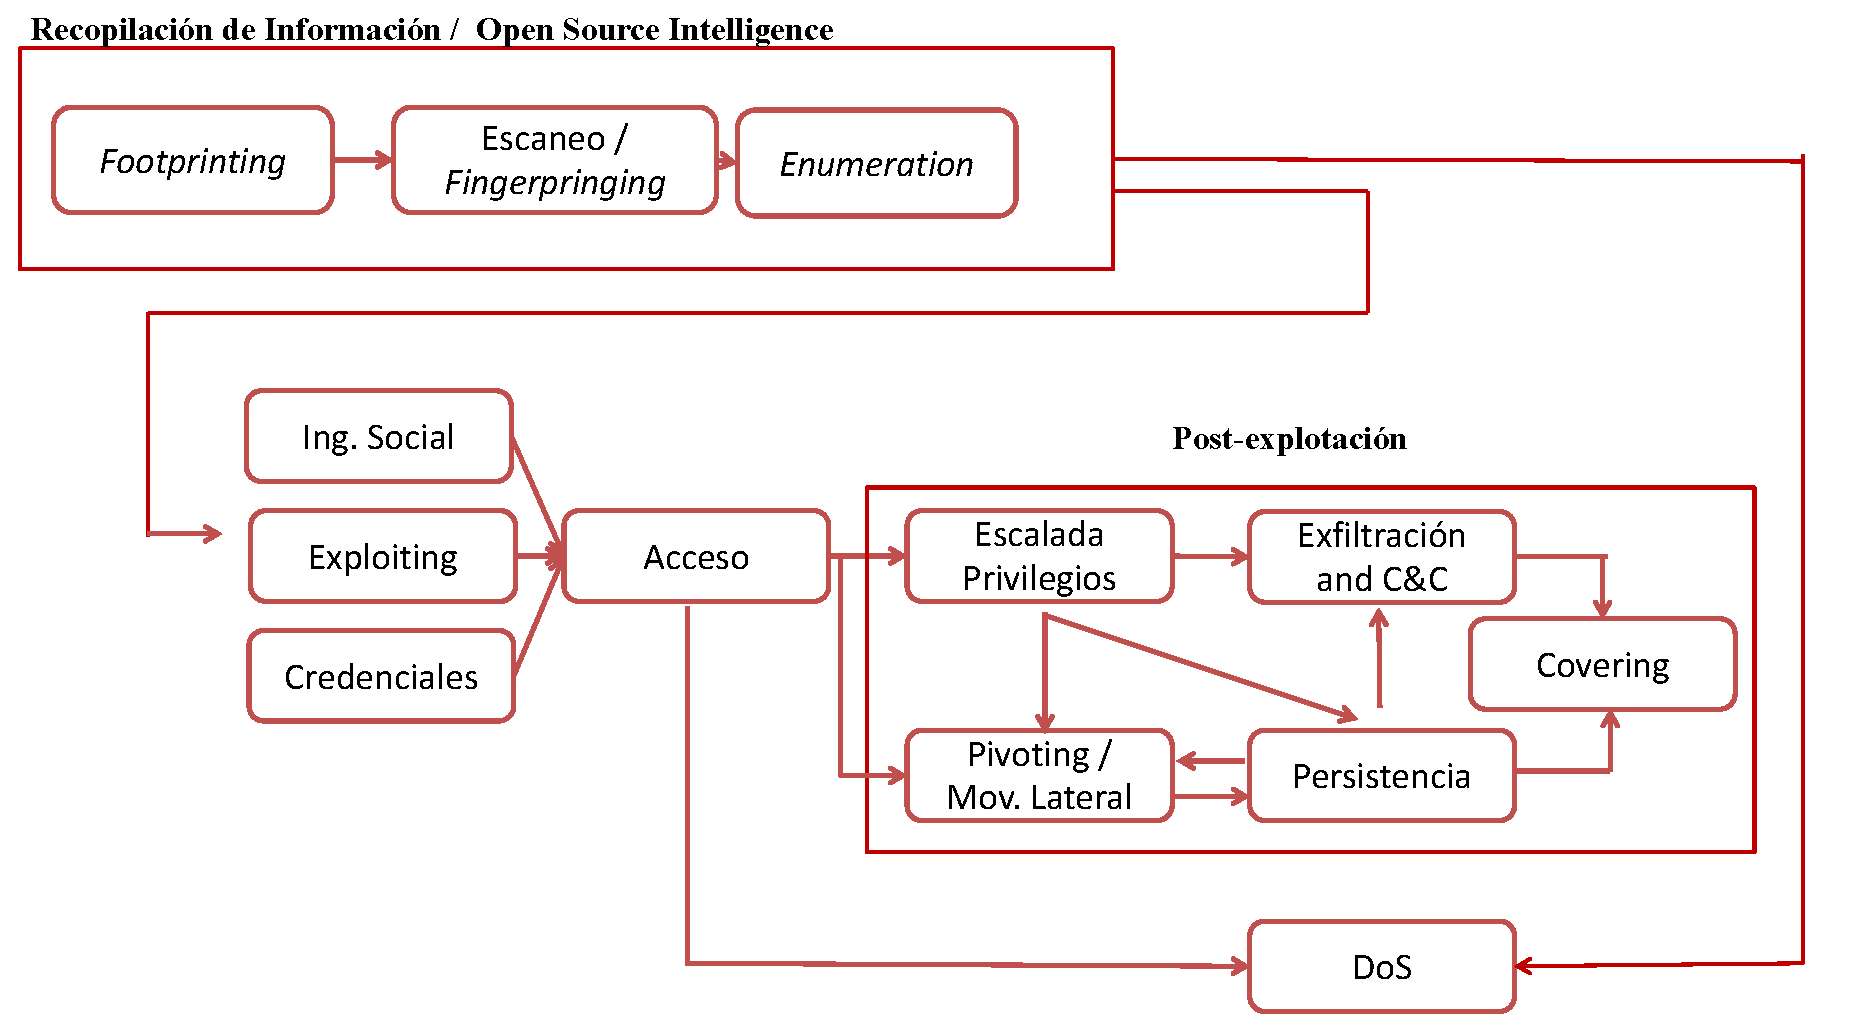
\includegraphics[width=\textwidth,height=0.82\textheight,keepaspectratio]{img/taxonomia-ataque.pdf}
\end{center}
\end{frame}

\begin{frame}[allowframebreaks]{Introducción}
\small
  \begin{itemize}
  \item Tras la fase de recopilación de información se habrán identificado la mayoría de los activos de la organización; entre ellos, servicios o aplicaciones que requieran un proceso de autenticación, por ejemplo: SSH, FTP, RDP, un CMS, dominios, etc.
  \item En un pentesting, cuyo objetivo es demostrar que el sistema es vulnerable a ataques de acceso, el vector de ataque o intrusión puede ser
  \begin{itemize}
  \item Aprovechar los propios servicios de acceso con autenticaciones débiles o ataques sobre estos (lo abordamos en este módulo 3.1)
  \item Utilizar técnicas de ingeniería social para conseguir credenciales válidas engañando al usuario o bien que ejecute algún payload camuflado de tipo RCE (lo veremos en el tema 3.2)
  \item Explotar una vulnerabilidad que permita la ejecución remota de código (se verá en el módulo 3.3)
  \end{itemize}
\end{itemize}
\end{frame}

\begin{frame}[allowframebreaks]{Introducción}
\small
\lead{Dentro de los ataques a las credenciales, se pueden identificar:}
  \begin{itemize}
  \item \textbf{Ataques online activos:} se interactúa con el servicio intentando averiguar el par \cmd{user:pass}
    \begin{itemize}
    \item Credenciales por defecto
    \item Reutilización de contraseñas
    \item Ataques de fuerza bruta
    \item Ataques basados en diccionario
    \item Malware (keylogger, spyware)
    \item Pass-the-Hash (es más de postexplotación --- pivoting)
    \end{itemize}
  \item \textbf{Ataques online pasivos:} se escuchan las comunicaciones y se esnifan credenciales válidas o sesiones activas (se verán en el módulo de sniffing)
    \begin{itemize}
    \item Session Replay (por ejemplo, a través de un XSS y robo de la cookie de sesión)
    \item Tablas rainbow
    \end{itemize}
  \item \textbf{Ataques no electrónicos:} los derivados de la ingeniería social, y los ataques online activos mejorados con ella (se verán en el tema 3.2)
  \end{itemize}
\end{frame}

\section{Ataques online activos}

\begin{frame}[allowframebreaks]{Credenciales por defecto}
\small
  \begin{itemize}
  \item En términos generales, los ataques a las credenciales consisten en averiguar el par \cmd{user:pass}. En una primera aproximación, si en la fase de fingerprinting hemos identificado un servicio o aplicación, podemos probar con las credenciales por defecto de dicho servicio o aplicación.
  \item Algunos repositorios para averiguar credenciales por defecto:
    \begin{itemize}
    \item \href{https://github.com/ihebski/DefaultCreds-cheat-sheet}{DefaultCreds-cheat-sheet}
    \item \href{https://github.com/danielmiessler/SecLists/blob/master/Passwords/Default-Credentials/default-passwords.csv}{SecLists --- Default Credentials}
    \item \href{https://github.com/Dormidera/WordList-Compendium}{WordList-Compendium}
    \item \href{https://www.cirt.net/passwords}{CIRT.net --- Default Passwords}
    \item \href{http://www.passwordsdatabase.com/}{passwordsdatabase.com}
    \item \href{https://datarecovery.com/rd/default-passwords/}{DataRecovery --- Default Passwords}
    \item \href{https://bizuns.com/default-passwords-list}{bizuns.com --- Default Passwords List}
    \item \href{https://192-168-1-1ip.mobi/default-router-passwords-list/}{Default Router Passwords List}
    \item \href{https://book.hacktricks.xyz/brute-force}{HackTricks --- Brute Force} (más repositorios)
    \end{itemize}
  \item Herramientas para comprobar credenciales por defecto:
    \begin{itemize}
    \item \href{https://github.com/ztgrace/changeme}{changeme}: a partir de una IP, identifica los puntos de autenticación y prueba credenciales por defecto
    \item \href{https://github.com/zricethezav/gitleaks}{gitleaks}: busca en repositorios de código contraseñas hardcodeadas, API keys, tokens, etc.
    \end{itemize}
  \end{itemize}
\end{frame}

\begin{frame}[allowframebreaks]{Reutilización de contraseñas}
\small
  \begin{itemize}
  \item Otra alternativa para comprometer un servicio de autenticación es comprobar la reutilización de credenciales.
  \item Un alto porcentaje de contraseñas, aun siendo seguras (no aparecen en diccionarios, contienen un espacio de caracteres elevado y una longitud robusta), son reutilizadas por parte de un mismo usuario en diferentes servicios o aplicaciones.
  \item Existen aplicaciones que buscan leaks de contraseñas de unos servicios para comprobar si esa contraseña se usa en otros.
  \item Sitios donde buscar leaks:
    \begin{itemize}
    \item \href{https://haveibeenpwned.com/}{Have I Been Pwned}: comprobación de correos electrónicos afectados por brechas de datos conocidas
    \item \href{https://monitor.mozilla.org/}{Mozilla Monitor}: monitorización de la exposición de direcciones de correo en filtraciones
    \item \href{https://dehashed.com/}{DeHashed}: motor de búsqueda de información procedente de filtraciones de datos
    \item \href{https://intelx.io/}{Intelligence X}: plataforma de inteligencia y búsqueda de información expuesta
    \item \href{https://breachdirectory.org/}{BreachDirectory}: consulta de información asociada a brechas de datos
    \item \href{https://www.google.com/}{Google} / \href{https://www.bing.com/}{Bing}: búsqueda de información expuesta o indexada públicamente
    \end{itemize}
  \item Herramientas:
    \begin{itemize}
    \item \href{https://github.com/D4Vinci/Cr3dOv3r}{Cr3dOv3r}: dado un correo, busca leaks conocidos y prueba las contraseñas encontradas en otros servicios
    \item \href{https://pwndb.com}{pwndb}: busca en la deep web filtraciones de datos con contraseñas de posibles usuarios
    \end{itemize}
  \item Contramedida: contraseñas únicas por servicio (gestor de contraseñas) y segundo factor (MFA). Véase la \href{https://cheatsheetseries.owasp.org/cheatsheets/Credential_Stuffing_Prevention_Cheat_Sheet.html}{OWASP Credential Stuffing Prevention Cheat Sheet}.
  \end{itemize}
\end{frame}

\section{Ataques de fuerza bruta}

\begin{frame}{Ataques fuerza bruta}
\small
  \begin{itemize}
  \item Otra alternativa es probar todas las combinaciones posibles, lo que se denomina ataques de fuerza bruta
  \item El tiempo de éxito es exponencial al tamaño de la clave y al espacio de caracteres que se usa
  \end{itemize}
\vfill
\begin{columns}[c]
  \begin{column}{0.38\textwidth}
    \centering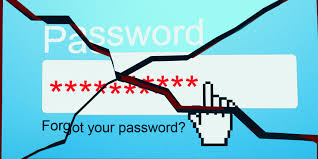
\includegraphics[width=\textwidth,height=0.40\textheight,keepaspectratio]{img/sl009_1.jpg}
  \end{column}
  \begin{column}{0.60\textwidth}
    \centering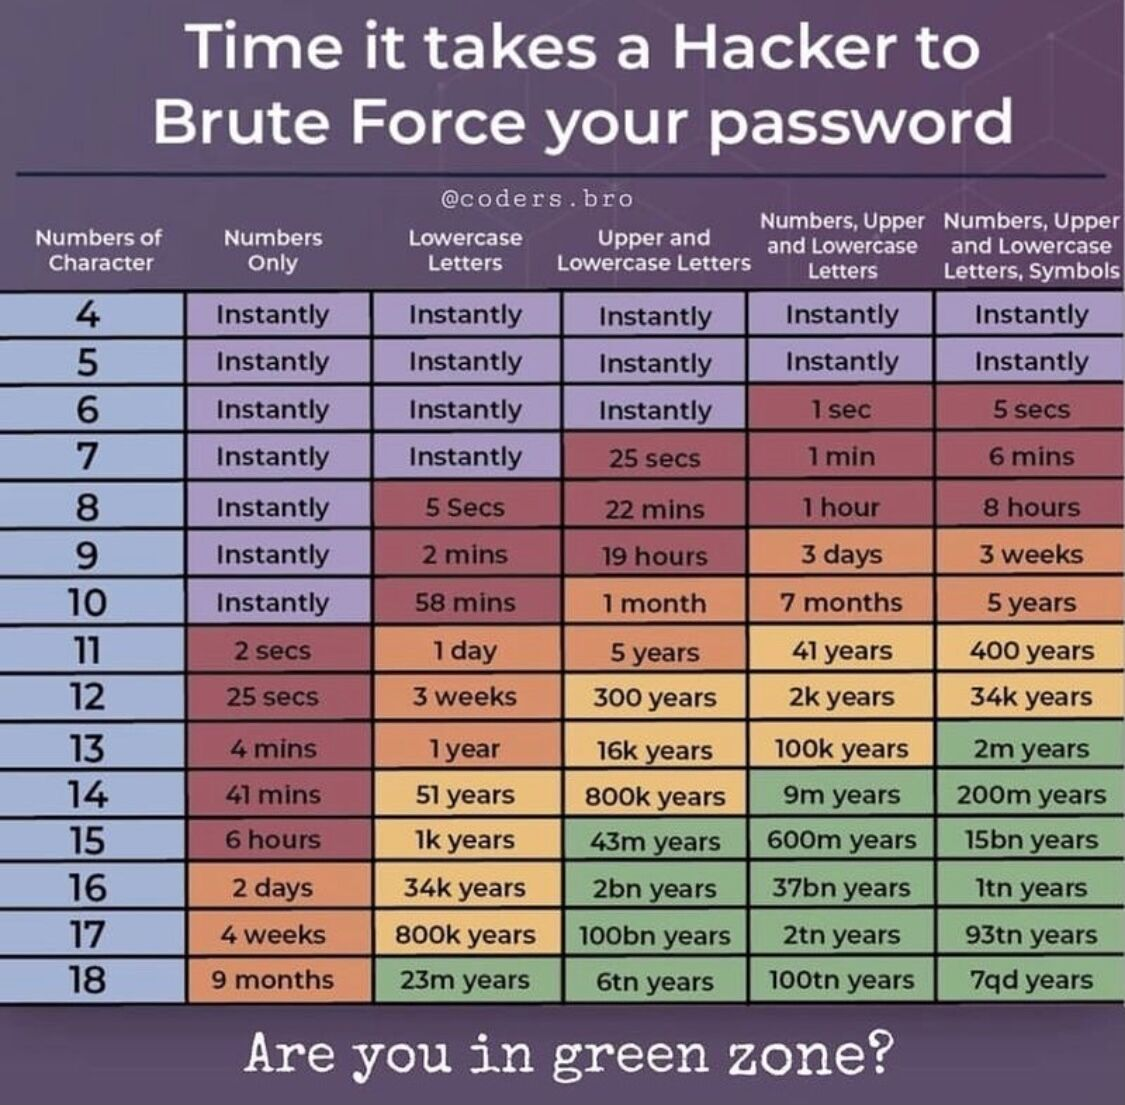
\includegraphics[width=\textwidth,height=0.60\textheight,keepaspectratio]{img/sl010_1.jpg}
  \end{column}
\end{columns}
\end{frame}

\begin{frame}{Ataques fuerza bruta}
\small
\lead{Ataques basados en diccionario}
\begin{columns}[T]
  \begin{column}{0.62\textwidth}
  \begin{itemize}
  \item Otra opción es probar con una combinación de usuarios y contraseñas definidas en un fichero, en lo que se denomina ataques basados en diccionario
  \item El éxito del ataque pasa por que la contraseña esté en el diccionario y por encontrar un usuario válido (enumeración)
  \item Diccionarios:
    \begin{itemize}
    \item RockYou, en \cmd{/usr/share/wordlists/}
      \begin{itemize}
      \item Descomprimir con \cmd{gunzip rockyou.txt.gz}
      \end{itemize}
    \item \href{https://github.com/kaonashi-passwords/Kaonashi}{Kaonashi}
    \item \href{https://github.com/danielmiessler/SecLists}{SecLists}
    \end{itemize}
  \end{itemize}
  \end{column}
  \begin{column}{0.36\textwidth}
    \centering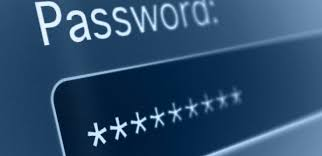
\includegraphics[width=\textwidth,height=0.55\textheight,keepaspectratio]{img/sl011_1.jpg}
  \end{column}
\end{columns}
\end{frame}

\begin{frame}[allowframebreaks]{Ataques fuerza bruta}
\small
\lead{Creación de diccionarios}
  \begin{itemize}
  \item \href{https://www.kali.org/tools/crunch/}{crunch}: genera diccionarios a partir de un patrón (longitud y juego de caracteres)
  \item \href{https://github.com/sc0tfree/mentalist}{Mentalist}: generador gráfico basado en reglas de mutación
  \item \href{https://github.com/hashcat/maskprocessor}{maskprocessor}: generador por máscaras, de los autores de Hashcat
  \item \href{https://github.com/LandGrey/pydictor}{pydictor}: generador y analizador de diccionarios
  \item \href{https://github.com/digininja/CeWL}{CeWL}: construye el diccionario con las palabras de una web (muy útil en CTFs)
  \item \href{https://github.com/t3l3machus/psudohash}{psudohash}: crea un diccionario a partir de otro aplicando mutaciones típicas, por ejemplo \cmd{Microsoft} $\rightarrow$ \cmd{M!cr0s0ft}
  \item \href{https://github.com/andreiverse/gorilla}{gorilla}: mezcla las capacidades de crunch, cupp, CeWL y las reglas de mutación
  \item Con ingeniería social (se verá en el tema 3.2): \href{https://github.com/Mebus/cupp}{cupp}, que construye el diccionario a partir de datos personales de la víctima
  \end{itemize}
\end{frame}

\begin{frame}[allowframebreaks]{Ataques fuerza bruta}
\small
  \begin{itemize}
  \item \href{https://github.com/brannondorsey/PassGAN}{PassGAN} es una herramienta de cracking basada en Redes Generativas Adversariales (GAN). Aprende la distribución estadística de contraseñas reales y genera candidatos nuevos, no incluidos en ningún diccionario.
  \item ¿Cómo funciona?
    \begin{itemize}
  \item Un generador (Generator) aprende patrones de millones de contraseñas reales filtradas (RockYou, LinkedIn\dots{})
  \item Un discriminador (Discriminator) evalúa si las contraseñas generadas parecen humanas
  \item El resultado: contraseñas estadísticamente plausibles que escapan a los diccionarios clásicos
    \end{itemize}
  \item Uso básico:
    \begin{itemize}\scriptsize
    \item \cmd{python3 passgan.py -{}-pretrained-model pretrained/gan.ckpt\\ -{}-output-file passwords.txt -n 1000000}
    \item \cmd{\# Genera 1M de candidatos; combinar luego con Hashcat o John}
    \end{itemize}
  \item Resultados y contexto:
    \begin{itemize}
    \item Reporta un 51--73\,\% más de contraseñas únicas frente a Hashcat + RockYou en ciertos datasets
    \item Más lento que Hashcat puro: es ideal para ataques dirigidos, no por volumen
    \item Tendencia: los modelos GAN y LLM aplicados a password cracking son cada vez más eficaces
    \end{itemize}
  \item Artículo original: Hitaj et al., \emph{PassGAN: A Deep Learning Approach for Password Guessing}, ACNS 2019 --- \href{https://arxiv.org/abs/1709.00440}{arXiv:1709.00440}
  \end{itemize}
\end{frame}




\begin{frame}[allowframebreaks]{Ataques fuerza bruta}
\small
\lead{Herramientas}
  \begin{itemize}
  \item \href{https://www.kali.org/tools/hydra/}{hydra} y \href{https://www.kali.org/tools/medusa/}{medusa}: fuerza bruta paralelizada contra decenas de protocolos de autenticación
    \begin{itemize}
    \item \cmd{hydra -l msfadmin -P rockyou.txt ssh://<IP>}
    \item \cmd{medusa -h <IP> -u msfadmin -P rockyou.txt -M ssh}
    \item \href{https://harshdushyants.medium.com/using-hydra-to-brute-force-different-services-3ea73470d213}{Ejemplo de uso frente a distintos servicios}
    \end{itemize}
  \end{itemize}
\begin{center}
\includegraphics[width=0.62\textwidth,height=0.42\textheight,keepaspectratio]{img/sl012_1.png}
\end{center}
\begin{center}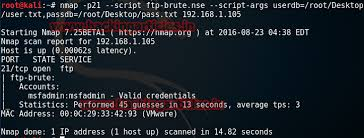
\includegraphics[width=0.62\textwidth,height=0.42\textheight,keepaspectratio]{img/sl012_2.jpg}
\end{center}
\end{frame}

\begin{frame}[allowframebreaks]{Ataques fuerza bruta}
\small
\lead{Herramientas}
  \begin{itemize}
  \item Nmap también hace fuerza bruta, con sus scripts NSE
  \item El motor \href{https://nmap.org/book/nse-usage.html}{NSE} incluye scripts \cmd{*-brute} para docenas de protocolos: útil cuando ya estás escaneando con Nmap y quieres auditar credenciales sin cambiar de herramienta. \href{https://www.hackingarticles.in/nmap-for-pentester-password-cracking/}{Ejemplo}
  \item Ejemplos por servicio:
    \begin{itemize}\scriptsize
    \item \cmd{nmap -p21 -{}-script ftp-brute -{}-script-args userdb=users.txt,passdb=pass.txt <IP>}
    \item \cmd{nmap -p22 -{}-script ssh-brute -{}-script-args userdb=users.txt,passdb=pass.txt <IP>}
    \item \cmd{nmap -p23 -{}-script telnet-brute -{}-script-args userdb=users.txt,passdb=pass.txt <IP>}
    \item \cmd{nmap -p445 -{}-script smb-brute -{}-script-args userdb=users.txt,passdb=pass.txt <IP>}
    \item \cmd{nmap -p3306 -{}-script mysql-brute -{}-script-args userdb=users.txt <IP>}
    \item \cmd{nmap -p5432 -{}-script pgsql-brute -{}-script-args userdb=users.txt,passdb=pass.txt <IP>}
    \item \cmd{nmap -p1433 -{}-script ms-sql-brute -{}-script-args userdb=users.txt,passdb=pass.txt <IP>}
    \item \cmd{nmap -p80 -{}-script http-form-brute\\ -{}-script-args "http-form-brute.path=/login" <IP>}
    \end{itemize}
  \item Descubrir todos los scripts de fuerza bruta:
    \begin{itemize}
    \item \cmd{locate *.nse | grep -i brute}
    \end{itemize}
  \item Los aciertos se guardan en el registro de Nmap (librería \cmd{creds}) para reutilizarlos en otros scripts
  \end{itemize}

\begin{center}
  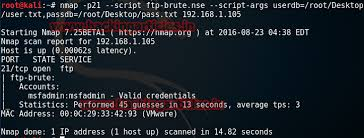
\includegraphics[width=0.62\textwidth,height=0.42\textheight,keepaspectratio]{img/sl012_2.jpg}
\end{center}
\end{frame}

\begin{frame}[allowframebreaks]{Ataques fuerza bruta}
\small
\lead{Herramientas}
  \begin{itemize}
  \item \href{https://www.metasploit.com/}{Metasploit} también dispone de varios módulos auxiliares para realizar ataques basados en diccionario frente a diferentes servicios
    \begin{itemize}
    \item \cmd{search type:auxiliary login}
    \item \cmd{use auxiliary/scanner/ssh/ssh\_login}
    \end{itemize}
  \end{itemize}
\begin{center}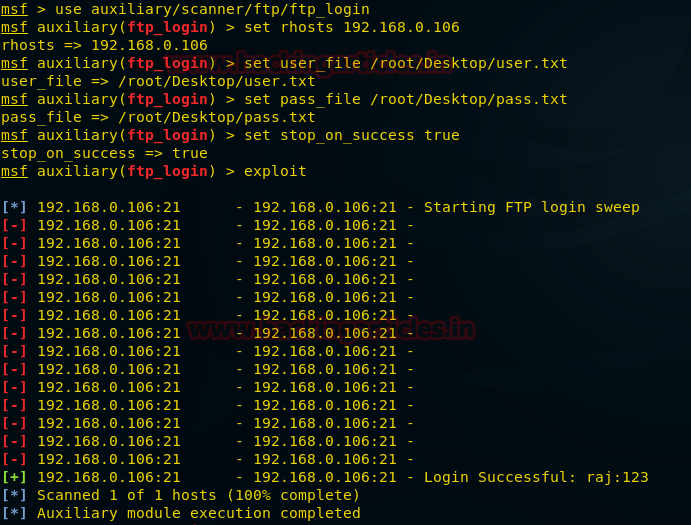
\includegraphics[width=0.78\textwidth,height=0.6\textheight,keepaspectratio]{img/sl013_1.png}
\end{center}
\end{frame}


\begin{frame}{Ejercicio}
\small
\begin{columns}[T]
  \begin{column}{0.62\textwidth}
  \begin{itemize}
  \item Realiza un ataque de diccionario frente a los servicios SSH y FTP de la máquina Metasploitable2, fijando como usuario \cmd{msfadmin} y usando un diccionario cualquiera de Kali
    \begin{itemize}
    \item Nota: puedes encontrar diccionarios en \cmd{/usr/share/wordlists/}
    \end{itemize}
  \item Realiza el ejercicio con las herramientas:
    \begin{itemize}
    \item hydra o medusa
    \item Metasploit
    \item NSE de Nmap
    \end{itemize}
  \end{itemize}
  \end{column}
  \begin{column}{0.36\textwidth}
    \centering
\includegraphics[width=\textwidth,height=0.55\textheight,keepaspectratio]{img/sl017_1.jpg}
  \end{column}
\end{columns}
\end{frame}

\begin{frame}{Ejercicio}
\small
\begin{center}
\includegraphics[width=0.78\textwidth,height=0.6\textheight,keepaspectratio]{img/sl018_1.jpg}
\end{center}
  \begin{itemize}
  \item Realiza un ataque de autenticación online (basado en diccionario) frente a la base de datos PostgreSQL de la distribución Metasploitable2 usando Metasploit
  \end{itemize}
\end{frame}

\begin{frame}{Ejercicio}
\small
\begin{columns}[T]
  \begin{column}{0.62\textwidth}
  \begin{itemize}
  \item Realiza un ataque de autenticación online (basado en diccionario) frente al servicio RDP (Remote Desktop Protocol) a un Windows, por ejemplo un \href{https://pruebasaluuclm-my.sharepoint.com/:u:/g/personal/joseluis_martinez_uclm_es/EZe0cefaSl9BgnV0-iw0eBQBGaPVrdQi5rC5RctPYDcv2Q?e=uuyf8A}{Win7}:
  \item \href{https://www.hackingarticles.in/remote-desktop-penetration-testing-port-3389/}{Ejemplo}
  \end{itemize}
  \end{column}
  \begin{column}{0.36\textwidth}
    \centering
\includegraphics[width=\textwidth,height=0.55\textheight,keepaspectratio]{img/sl019_1.jpg}
  \end{column}
\end{columns}
\end{frame}

\begin{frame}{Ejercicio}
\small
¡Nivel Examen!
\begin{columns}[T]
  \begin{column}{0.62\textwidth}
  \begin{itemize}
  \item Resuelve la máquina \href{https://tryhackme.com/room/poster}{Poster} de TryHackMe, necesitarás:
    \begin{itemize}
    \item Escanear
    \item Usa metasploit para enumerar en el postgres
    \item Usa metasploit para hacer fuerza bruta al postgres
    \end{itemize}
  \item Nota: Para elevar privilegios en la máquina root hacerlo como ejercicio del tema de postexplotación
  \end{itemize}
  \end{column}
  \begin{column}{0.36\textwidth}
    \centering
\includegraphics[width=\textwidth,height=0.55\textheight,keepaspectratio]{img/sl020_1.jpg}
  \end{column}
\end{columns}
\end{frame}

\begin{frame}[allowframebreaks]{Ataques fuerza bruta}
\small
\lead{Fuerza bruta contra un login web}
  \begin{itemize}
  \item Hacer ataques de fuerza bruta o de diccionario contra un panel o login web no es tan trivial como hacerlo frente a servicios SSH, Telnet, MySQL, etc.
  \item ¿Por qué? Dichos servicios llevan el proceso de autenticación implementado de manera intrínseca en el propio protocolo. Las herramientas simplemente implementan el protocolo y cambian el par \cmd{user:pass} en cada petición al servicio.
  \item El problema viene al hacer esto frente a una aplicación o formulario web, ya que el protocolo HTTP/HTTPS no lleva de manera intrínseca el proceso de autenticación: quien lo implementa es la propia aplicación web.
  \item Por tanto, debemos comunicarnos con la lógica de la aplicación usando HTTP/HTTPS. Para ello hay que ver cómo se construye la petición que envía el navegador (usuario) al servidor (aplicación web) y parametrizarla con diferentes usuarios y contraseñas.
  \item Para hacer esto nos apoyamos en proxies web como \href{https://portswigger.net/burp}{Burp Suite} o \href{https://www.zaproxy.org/}{OWASP ZAP}. En el caso de Burp Suite, en la pestaña \emph{Intruder}:
    \begin{itemize}
    \item Nos ponemos en medio entre el navegador y la aplicación web (proxy), usando la configuración de red del propio navegador
    \item Redirigimos las peticiones al puerto \cmd{8080}, que es donde está escuchando Burp
    \item Capturamos la petición de autenticación y la enviamos a la pestaña \emph{Intruder}
    \item Desde \emph{Intruder}, parametrizamos el usuario y/o la contraseña usando un diccionario a nuestra elección
    \item \href{https://www.hackingarticles.in/wordlists-for-pentester/}{Lectura recomendable}
    \end{itemize}
  \end{itemize}
\begin{center}
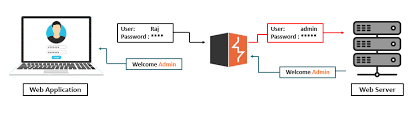
\includegraphics[width=0.62\textwidth,height=0.42\textheight,keepaspectratio]{img/sl021_2.png}
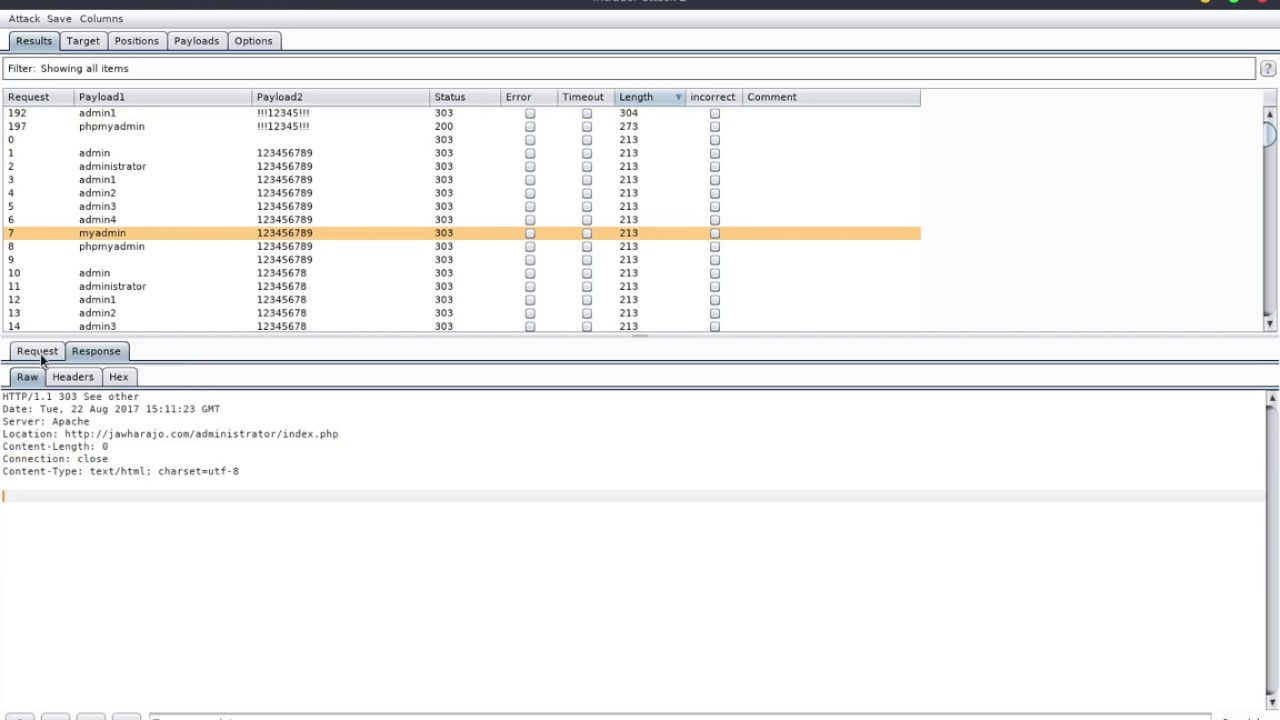
\includegraphics[width=0.62\textwidth,height=0.42\textheight,keepaspectratio]{img/sl021_1.jpg}
\end{center}
\end{frame}

\begin{frame}{Ejercicio}
\small
\begin{columns}[T]
  \begin{column}{0.62\textwidth}
  \begin{itemize}
  \item Realiza un ataque de diccionario a la aplicación web DVWA que viene alojada en la distribución Metasploitable2, frente al login web
    \begin{itemize}
    \item Las credenciales son \cmd{admin/password}
    \end{itemize}
  \end{itemize}
  \end{column}
  \begin{column}{0.36\textwidth}
    \centering
\includegraphics[width=\textwidth,height=0.55\textheight,keepaspectratio]{img/sl022_1.jpg}
  \end{column}
\end{columns}
\end{frame}

\begin{frame}{Ejercicio}
\small
\begin{center}
\includegraphics[width=0.78\textwidth,height=0.6\textheight,keepaspectratio]{img/sl023_1.jpg}
\end{center}
  \begin{itemize}
  \item Realiza el mismo ejercicio anterior, pero con la herramienta hydra
  \end{itemize}
\end{frame}

\begin{frame}{Ejercicio}
\small
\begin{center}
\includegraphics[width=0.78\textwidth,height=0.6\textheight,keepaspectratio]{img/sl024_1.jpg}
\end{center}
  \begin{itemize}
  \item Realiza un ataque de diccionario a la aplicación web DVWA que viene alojada en la distribución Metasploitable2, en concreto a la pestaña ``Brute Force'' que hay en el índice
  \end{itemize}
\end{frame}

\begin{frame}{Ejercicio}
\small
\begin{columns}[T]
  \begin{column}{0.62\textwidth}
  \begin{itemize}
  \item Resuelve la máquina \href{https://dockerlabs.es/}{StrongJenkins} de DockerLabs
    \begin{itemize}
    \item Fuerza bruta con RockYou en Jenkins (usuario \cmd{admin}; la contraseña hay que obtenerla por fuerza bruta)
    \item Divide el RockYou en trozos para que lo digiera mejor:
      \begin{itemize}
      \item \cmd{split -n l/20 rockyou.txt diccionario\_}
      \end{itemize}
    \end{itemize}
  \end{itemize}
  \end{column}
  \begin{column}{0.36\textwidth}
    \centering
\includegraphics[width=\textwidth,height=0.55\textheight,keepaspectratio]{img/sl025_1.jpg}
  \end{column}
\end{columns}
\end{frame}

\begin{frame}{Ejercicio}
\small
\begin{center}
\includegraphics[width=0.78\textwidth,height=0.6\textheight,keepaspectratio]{img/sl026_1.jpg}
\end{center}
  \begin{itemize}
  \item Resuelve la room de TryHackMe sobre \href{https://tryhackme.com/r/room/hydra}{hydra}
  \end{itemize}
\end{frame}

\begin{frame}{Ejercicio}
\small
\begin{center}
\includegraphics[width=0.78\textwidth,height=0.6\textheight,keepaspectratio]{img/sl027_1.jpg}
\end{center}
  \begin{itemize}
  \item Prueba la herramienta hydra en otras situaciones o contextos, como algunos de los que aparecen \href{https://pruebasaluuclm-my.sharepoint.com/:b:/g/personal/joseluis_martinez_uclm_es/ETAsVF1pUWRAglKv26ADbDsBCxLoDud8LDmnhz7vBDtFNg?e=c41GbV}{en este documento}
  \end{itemize}
\end{frame}

\begin{frame}[allowframebreaks]{Ataques fuerza bruta}
\small
\lead{Ataque por diccionario al login de WordPress}
  \begin{itemize}
  \item El panel de acceso suele estar en \cmd{/wp-admin/} o \cmd{/wp-login.php}
  \item Herramientas específicas:
    \begin{itemize}
    \item \href{https://wpscan.com/wordpress-security-scanner}{WPScan}: enumera usuarios, plugins y temas, y hace fuerza bruta contra el login
      \begin{itemize}
      \item \cmd{wpscan -{}-url http://<IP>/ -{}-enumerate u}
      \item \cmd{wpscan -{}-url http://<IP>/ -U admin -P rockyou.txt}
      \end{itemize}
    \item \href{https://github.com/andripwn/WPSeku}{WPSeku}: escáner de vulnerabilidades para WordPress
    \end{itemize}
  \end{itemize}
\end{frame}

\begin{frame}{Ejercicio}
\small
\begin{columns}[T]
  \begin{column}{0.62\textwidth}
  \begin{itemize}
  \item Puedes probar a hacer fuerza bruta frente a un WordPress en las máquinas
  \begin{itemize}
    \item Máquina leemonsqueezy (ya la vimos en enumeración y la veremos en postexplotación)
    \item Máquina Loly (la veremos también en postexplotación)
  \end{itemize}
  \end{itemize}
  \end{column}
  \begin{column}{0.36\textwidth}
    \centering
\includegraphics[width=\textwidth,height=0.55\textheight,keepaspectratio]{img/sl027_1.jpg}
  \end{column}
\end{columns}
\end{frame}

\section{Malware}

\begin{frame}[allowframebreaks]{Malware}
\small
\lead{Keylogger}
  \begin{itemize}
  \item Es un tipo de malware (software malicioso), o un dispositivo hardware específico, que se encarga de registrar las pulsaciones que se realizan en el teclado
  \item Se usa para robar credenciales válidas, tarjetas de crédito, PIN, etc.
  \item Los de tipo software se instalan vía troyano, phishing, etc., y los de tipo hardware requieren una instalación manual
  \item Este tipo de ataques se suele usar en combinación con técnicas de ingeniería social para potenciar el alcance y la efectividad del ataque (se verá en el tema 3.2)
  \item En MITRE ATT\&CK se corresponde con la técnica \href{https://attack.mitre.org/techniques/T1056/001/}{T1056.001 --- Keylogging}
  \end{itemize}
\end{frame}

\begin{frame}[allowframebreaks]{Malware}
\small
\lead{Keylogger software vs. keylogger hardware}
\begin{center}
\includegraphics[width=0.62\textwidth,height=0.42\textheight,keepaspectratio]{img/sl030_1.png}
\end{center}
\begin{center}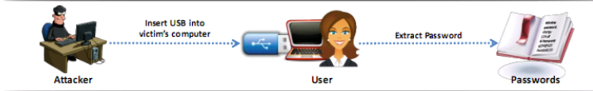
\includegraphics[width=0.62\textwidth,height=0.42\textheight,keepaspectratio]{img/sl030_2.png}
\end{center}
\end{frame}

\section{Ataques offline}

\begin{frame}[allowframebreaks]{Ataques offline}
\small
  \begin{itemize}
  \item Los ataques offline se refieren a las técnicas y herramientas que intentan ``romper'' una clave cifrada o hasheada.
  \item Un algoritmo hash no tiene inversa: el proceso de generar el resumen es unidireccional y, dado un resumen, es computacionalmente imposible determinar la entrada que lo generó.
  \item El atacante hace el proceso inverso por prueba y comparación: cuando encuentra una coincidencia, ha encontrado una contraseña candidata que produce ese hash.
  \item Estas herramientas se apoyan en \emph{tablas rainbow}, que no son más que tablas precomputadas que sirven a modo de diccionario. Es decir, son diccionarios previamente hasheados o cifrados con diferentes algoritmos; basta con comparar el hash objetivo con la tabla y, si coincide, ya se tiene la contraseña.
  \item En Windows, el concepto aparece asociado a las credenciales almacenadas en la \cmd{SAM} o en \cmd{NTDS.dit} (MITRE ATT\&CK \href{https://attack.mitre.org/techniques/T1003/}{T1003 --- OS Credential Dumping}).
  \end{itemize}
\end{frame}

\begin{frame}{Ataques offline}
\small
\lead{¿Qué es el salt?}
  \begin{itemize}
  \item Es un valor aleatorio que se añade a una contraseña antes de calcular su hash.
  \item Sirve para evitar que dos usuarios con la misma contraseña tengan el mismo hash y dificulta enormemente el uso de tablas precalculadas (rainbow tables).
  \item El salt \textbf{no} tiene que mantenerse secreto: normalmente se almacena junto al hash. La seguridad viene de que sea aleatorio y diferente para cada contraseña, no de ocultarlo.
  \item Referencia: \href{https://cheatsheetseries.owasp.org/cheatsheets/Password_Storage_Cheat_Sheet.html}{OWASP Password Storage Cheat Sheet}.
  \end{itemize}
\end{frame}

\begin{frame}{Ataques offline}
\small
\lead{Algoritmos de hash y almacenamiento de contraseñas}
Aparecieron vulnerabilidades en MD5 (los llamados ataques de colisión), que en ciertas circunstancias permiten obtener una entrada cualquiera dado un resumen. Algoritmos recomendados:
\begin{center}
\begin{tabular}{ll}
    \toprule
    \textbf{Algoritmo} & \textbf{Uso para contraseñas} \\
    \midrule
    MD5              & Obsoleto \\
    SHA-1            & Obsoleto \\
    SHA-256 directo  & No recomendado para almacenar contraseñas \\
    PBKDF2           & Adecuado con parámetros apropiados \\
    bcrypt           & Adecuado \\
    scrypt           & Adecuado \\
    Argon2id         & Muy recomendado (\href{https://www.rfc-editor.org/rfc/rfc9106.html}{RFC 9106}) \\
    \bottomrule
\end{tabular}
\end{center}
\medskip
Véase también \href{https://pages.nist.gov/800-63-3/sp800-63b.html}{NIST SP 800-63B --- Digital Identity Guidelines}.
\end{frame}

\begin{frame}[allowframebreaks]{Ataques offline}
\small
\lead{Criptografía simétrica: ¿cómo se ataca?}
  \begin{itemize}
  \item Normalmente no se ``rompe'' el algoritmo (AES, ChaCha20, etc.). En la práctica, los ataques intentan obtener la clave o aprovechar una mala implementación:
  \begin{itemize}
    \item \textbf{Fuerza bruta de la clave:} probar sistemáticamente posibles claves hasta encontrar la correcta. Solo es viable cuando la clave es suficientemente pequeña o débil.

    \item \textbf{Claves débiles o derivadas de contraseñas:} atacar la contraseña de la que se obtiene la clave mediante diccionarios, reglas o fuerza bruta.

    \item \textbf{Fugas de claves:} localizar las claves en código fuente, ficheros de configuración, variables de entorno, logs, copias de seguridad, repositorios o memoria.

    \item \textbf{Errores en la implementación:} explotar una utilización incorrecta del algoritmo, por ejemplo, reutilización de IV/nonce, generación de números aleatorios predecibles o una gestión deficiente de claves.

    \item \textbf{Debilidades del modo de operación:} determinadas configuraciones pueden permitir ataques que revelen o permitan modificar información sin necesidad de romper directamente el algoritmo criptográfico.

    \item \textbf{Ataques criptanalíticos:} aprovechar vulnerabilidades matemáticas conocidas en algoritmos concretos o en determinadas configuraciones.

    \item \textbf{Side-channel attacks:} obtener información sobre la clave analizando características físicas de la ejecución, como tiempos de ejecución, consumo de energía o emisiones electromagnéticas.

    \item \textbf{Compromiso del sistema:} obtener la clave desde un sistema que ya ha sido comprometido, evitando tener que atacar el algoritmo criptográfico.
\end{itemize}

\end{itemize}
\end{frame}

\begin{frame}{Ataques offline}
\small
\lead{Criptografía simétrica: opciones más seguras}
\begin{itemize}
    \item \textbf{AES-256:} opción estándar, ampliamente analizada y recomendada para cifrado simétrico.
    
    \item \textbf{AES-GCM:} modo AEAD que proporciona simultáneamente confidencialidad e integridad (autenticación del mensaje).
    
    \item \textbf{ChaCha20-Poly1305:} alternativa moderna a AES-GCM, especialmente interesante en dispositivos sin aceleración AES por hardware.
    
    \item \textbf{XChaCha20-Poly1305:} variante de ChaCha20-Poly1305 con un nonce más largo, útil para reducir el riesgo de colisiones de nonce.
\end{itemize}
\end{frame}

\begin{frame}[allowframebreaks]{Ataques offline}
\small
\lead{Criptografía asimétrica: ¿cómo se ataca?}
\begin{itemize}
    \item \textbf{Fuerza bruta:} búsqueda exhaustiva de la clave privada; impracticable con tamaños de clave adecuados.
    
    \item \textbf{Claves débiles o pequeñas:} tamaños insuficientes pueden permitir ataques criptográficos.
    
    \item \textbf{Algoritmos obsoletos:} algoritmos que ya no proporcionan un nivel de seguridad adecuado.
    
    \item \textbf{Exposición de la clave privada:} robo desde ficheros, backups, repositorios, memoria o dispositivos.
    
    \item \textbf{Contraseñas débiles:} ataque offline contra la contraseña que protege una clave privada.
    
    \item \textbf{Generación deficiente de claves:} números aleatorios predecibles o parámetros incorrectamente generados.
    
    \item \textbf{Errores de implementación:} fallos en la implementación del algoritmo o de los protocolos criptográficos.
    
    \item \textbf{Ataques de canal lateral:} extracción indirecta de información sobre la clave mediante tiempos, consumo, cachés u otras señales.
    
    \item \textbf{Ataques al protocolo:} explotación de una utilización incorrecta de la criptografía dentro de protocolos como TLS o SSH.
    
    \item \textbf{Criptoanálisis:} explotación de debilidades matemáticas del algoritmo o de su configuración.
    
    \item \textbf{Ataques cuánticos:} algoritmos como Shor podrían comprometer RSA y ECC cuando existan ordenadores cuánticos suficientemente potentes.
\end{itemize}
\end{frame}

\begin{frame}{Ataques offline}
\small
\lead{Criptografía asimétrica: alternativas más seguras}
\begin{itemize}
    \item \textbf{X25519:} recomendado para intercambio de claves basado en curvas elípticas.

    \item \textbf{Ed25519:} recomendado para firmas digitales, con buen rendimiento y claves compactas.

    \item \textbf{ECDH/ECDSA:} alternativas ampliamente utilizadas para intercambio de claves y firmas digitales, respectivamente.

    \item \textbf{RSA-2048 o superior:} todavía válido cuando se requiere compatibilidad con sistemas existentes, aunque ECC suele ser preferible en nuevos diseños.

    \item \textbf{ML-KEM (Kyber):} mecanismo de encapsulación de claves estandarizado para criptografía poscuántica.

    \item \textbf{ML-DSA (Dilithium):} algoritmo de firma digital poscuántica estandarizado.
\end{itemize}
\end{frame}


\begin{frame}[allowframebreaks]{Ataques offline}
\small

  \begin{itemize}

\item En este tema nos vamos a centrar en cómo romper claves hasheadas.
\item Para ello, disponemos de las siguientes herramientas:
  \begin{itemize}
  \item \href{https://www.openwall.com/john/doc/}{John the Ripper} (\href{https://www.redeszone.net/seguridad-informatica/john-the-ripper-crackear-contrasenas/}{tutorial en castellano})
    \begin{itemize}
    \item \cmd{john -{}-wordlist=rockyou.txt hashes.txt}
    \item \cmd{john -{}-show hashes.txt}
    \end{itemize}
  \item \href{https://hashcat.net/wiki/}{Hashcat}, que aprovecha la GPU (\href{https://blog.elhacker.net/2020/02/crackear-contrasenas-windows-ntlm-de-8-caracteres-en-menos-de-2-horas-y-media.html}{ejemplo con NTLM})
    \begin{itemize}
    \item \cmd{hashcat -m 0 -a 0 hashes.txt rockyou.txt}
    \end{itemize}
  \item Identificar el algoritmo del hash:
    \begin{itemize}
    \item \href{https://github.com/psypanda/hashID}{hashid} y \href{https://www.kali.org/tools/hash-identifier/}{hash-identifier}
    \end{itemize}
  \item Calcular hashes o cifrar con diferentes algoritmos:
    \begin{itemize}
    \item \href{https://www.openssl.org/}{openssl}, por ejemplo \cmd{echo -n password | openssl dgst -sha256}
    \end{itemize}
  \end{itemize}
\item Técnica MITRE ATT\&CK asociada: \href{https://attack.mitre.org/techniques/T1110/}{T1110.002 --- Password Cracking}
    \end{itemize}

\begin{center}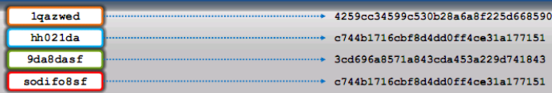
\includegraphics[width=0.78\textwidth,height=0.6\textheight,keepaspectratio]{img/sl034_1.png}
\end{center}
\end{frame}

\begin{frame}{Ataques offline}
\begin{columns}[c]
  \begin{column}{0.58\textwidth}
    \centering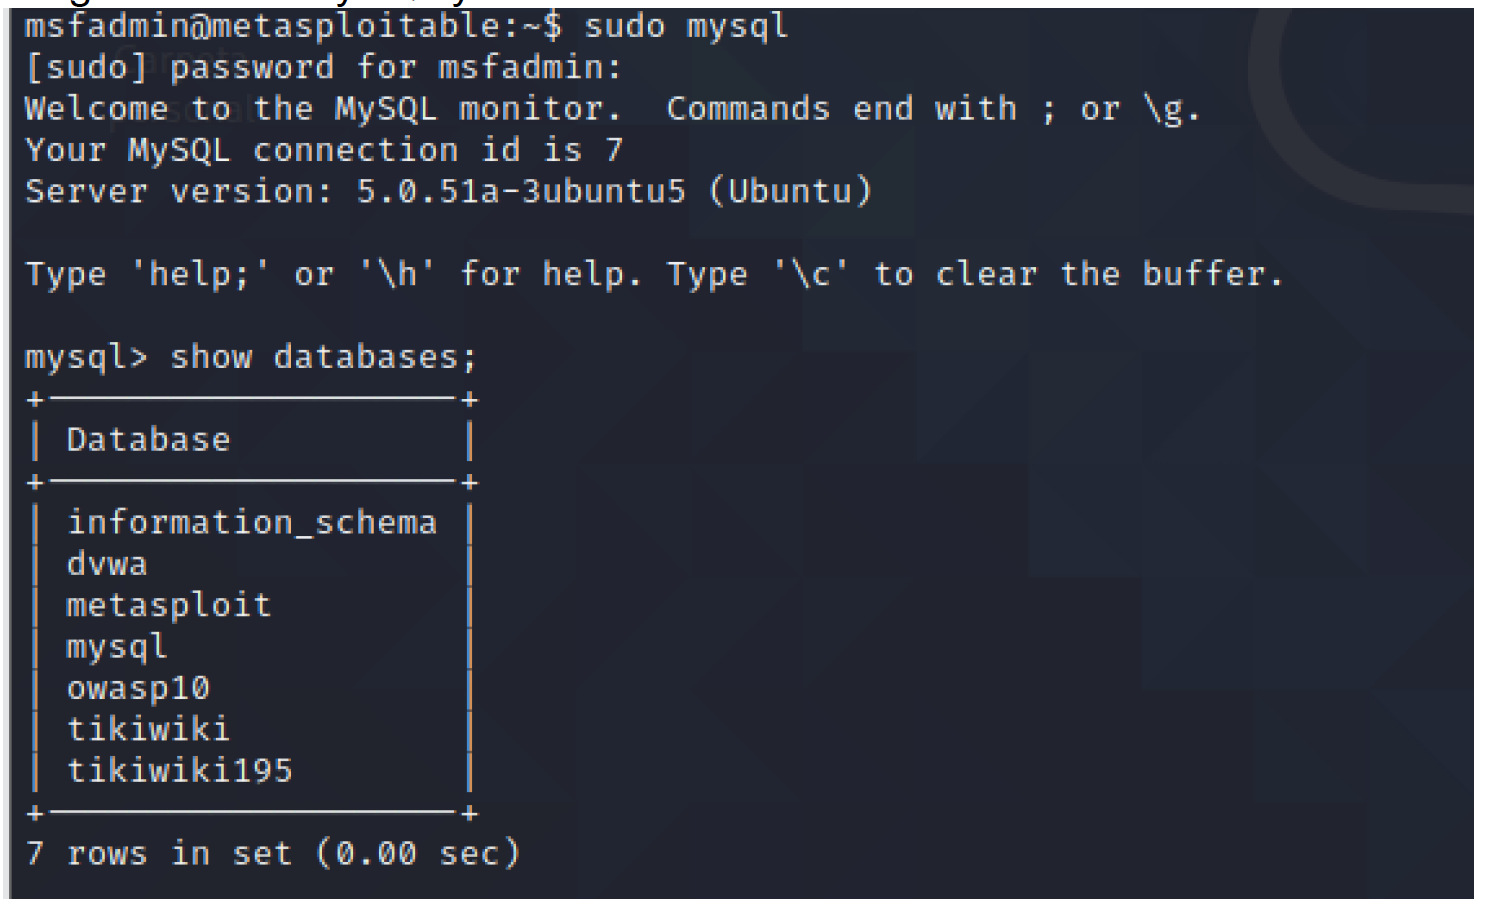
\includegraphics[width=\textwidth,height=0.70\textheight,keepaspectratio]{img/sl035_1.png}
  \end{column}
  \begin{column}{0.40\textwidth}
    \centering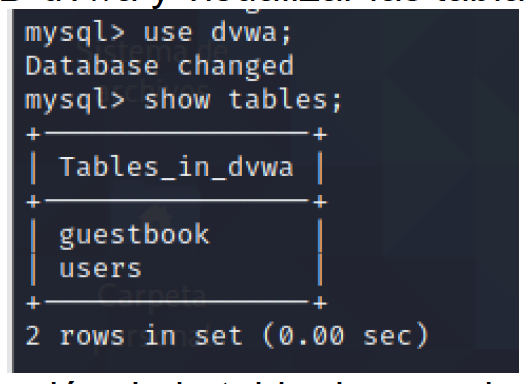
\includegraphics[width=\textwidth,height=0.50\textheight,keepaspectratio]{img/sl035_2.png}
  \end{column}
\end{columns}
\end{frame}

\begin{frame}{Ataques offline}
\begin{center}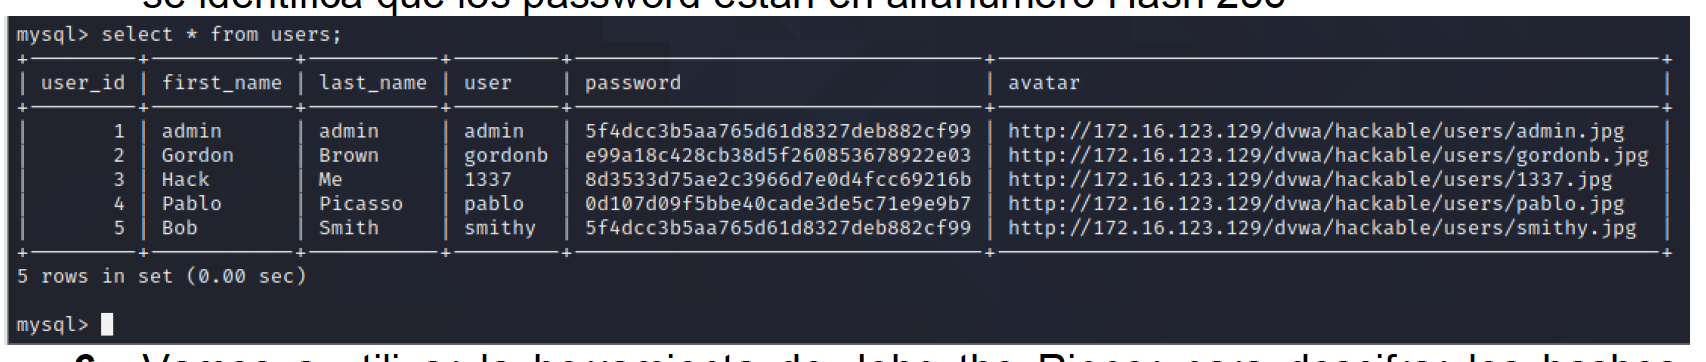
\includegraphics[width=0.95\textwidth,height=0.32\textheight,keepaspectratio]{img/sl035_3.png}
\end{center}
\vfill
\begin{center}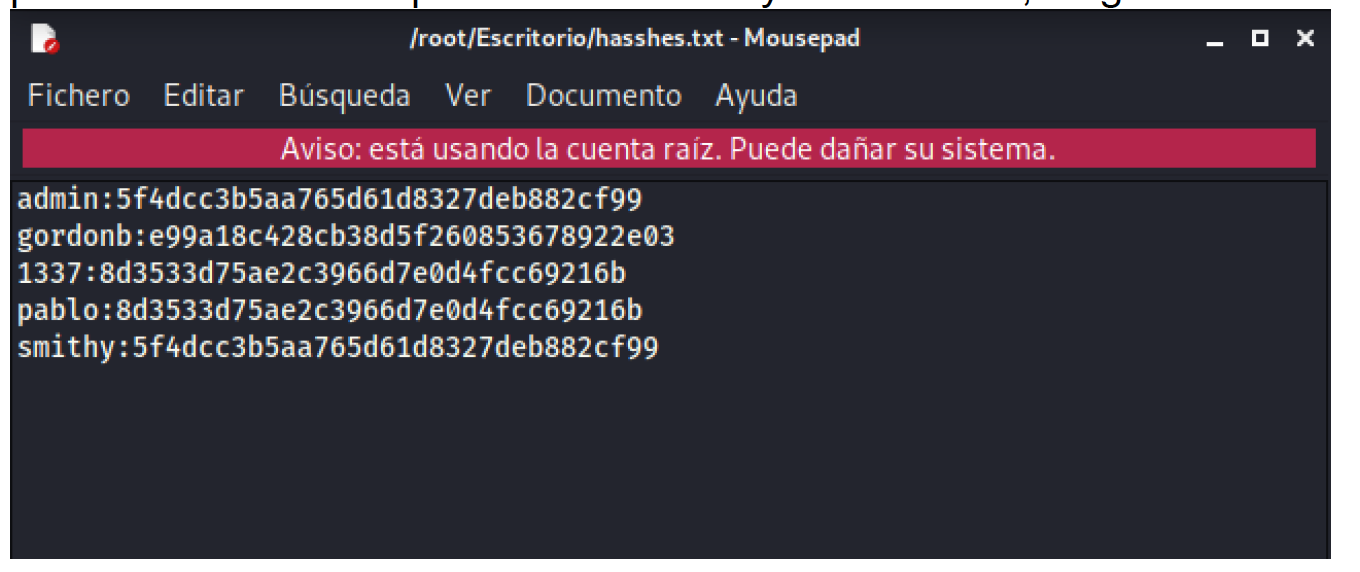
\includegraphics[width=0.70\textwidth,height=0.42\textheight,keepaspectratio]{img/sl036_1.png}
\end{center}
\end{frame}

\begin{frame}{Ataques offline}
\begin{center}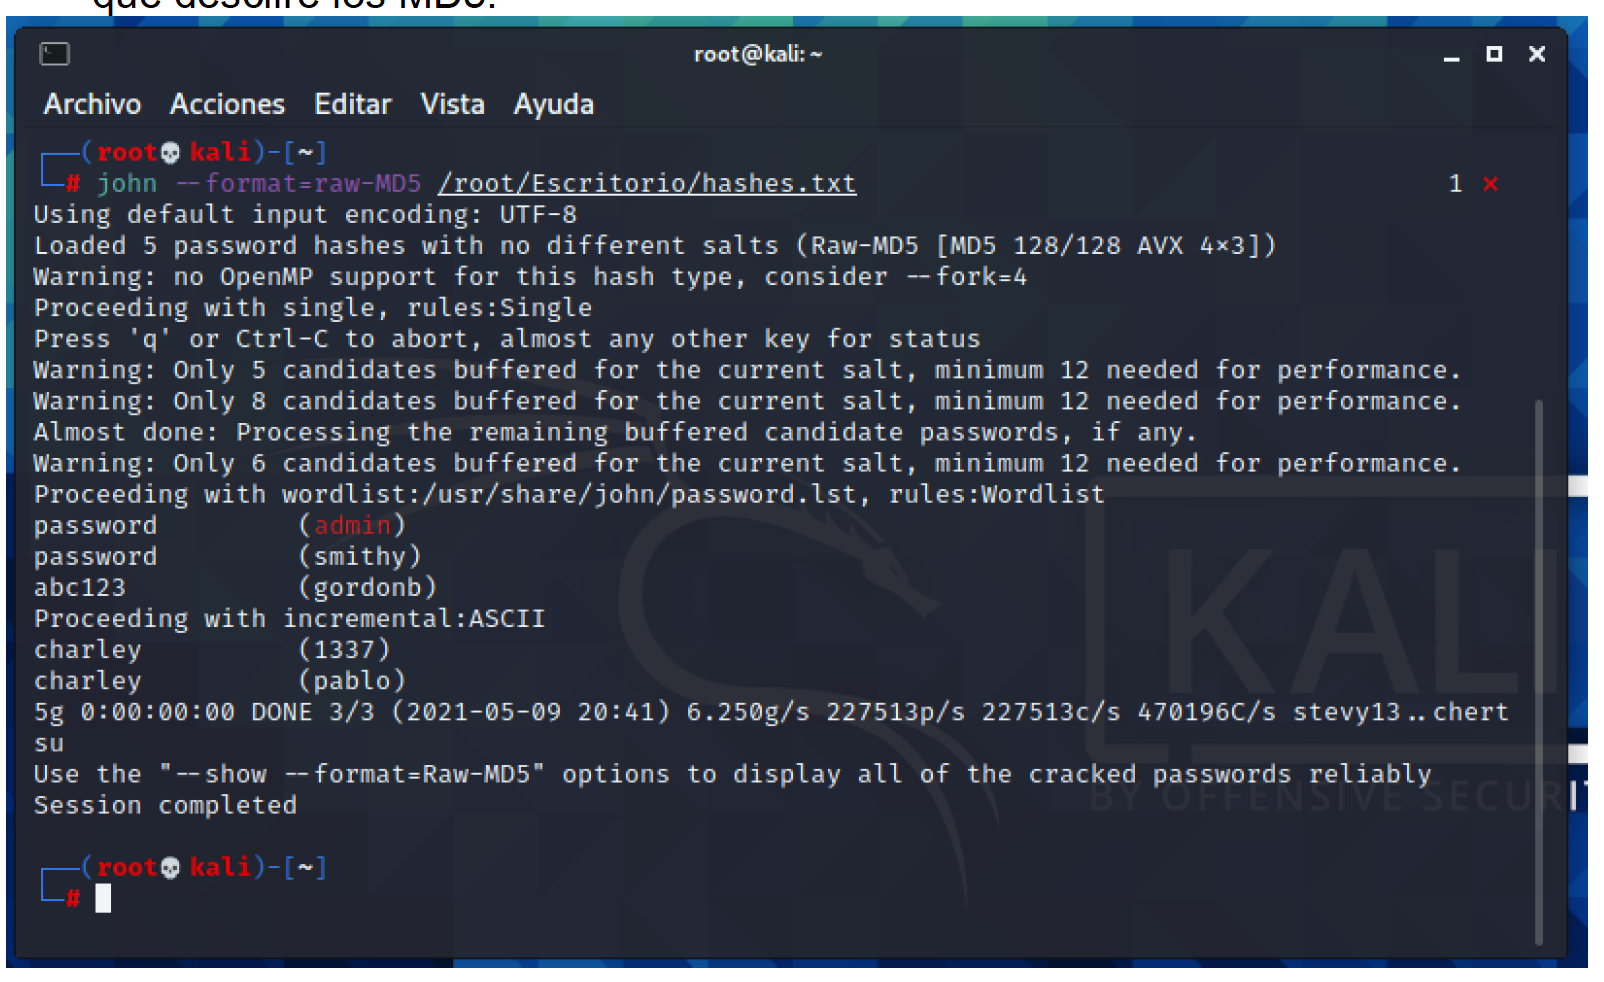
\includegraphics[width=0.80\textwidth,height=0.80\textheight,keepaspectratio]{img/sl036_2.png}
\end{center}
\end{frame}

\begin{frame}[allowframebreaks]{Ejercicio}
\begin{center}
\includegraphics[width=0.78\textwidth,height=0.6\textheight,keepaspectratio]{img/sl037_1.jpg}
\end{center}
Conéctate de manera remota a la BBDD MySQL de Metasploitable2, accede a las contraseñas almacenadas y recupera las claves en claro.
\end{frame}

\begin{frame}[allowframebreaks]{Ataques offline}
\small
\lead{El mismo ejercicio con Metasploit}
  \begin{itemize}
  \item Módulos auxiliares para MySQL:
    \begin{itemize}
    \item \cmd{auxiliary/admin/mysql/mysql\_sql} \# ejecutar SQL (\cmd{show databases;})
    \item \cmd{auxiliary/scanner/mysql/mysql\_schemadump} \# volcar el esquema completo
    \item \cmd{auxiliary/scanner/mysql/mysql\_hashdump} \# usuarios + hashes
    \end{itemize}
  \item Con \cmd{root/123} se enumeran las bases de datos, se vuelca todo el esquema y se extraen los hashes de los usuarios MySQL (crackeables después con John o Hashcat)
  \item Hacia RCE:
    \begin{itemize}
    \item \cmd{auxiliary/scanner/mysql/mysql\_writable\_dirs} \# directorios escribibles
    \item Con \cmd{secure\_file\_priv} vacío y privilegio \cmd{FILE} $\rightarrow$ escribir ficheros (webshell o UDF)
    \end{itemize}
  \end{itemize}
\begin{center}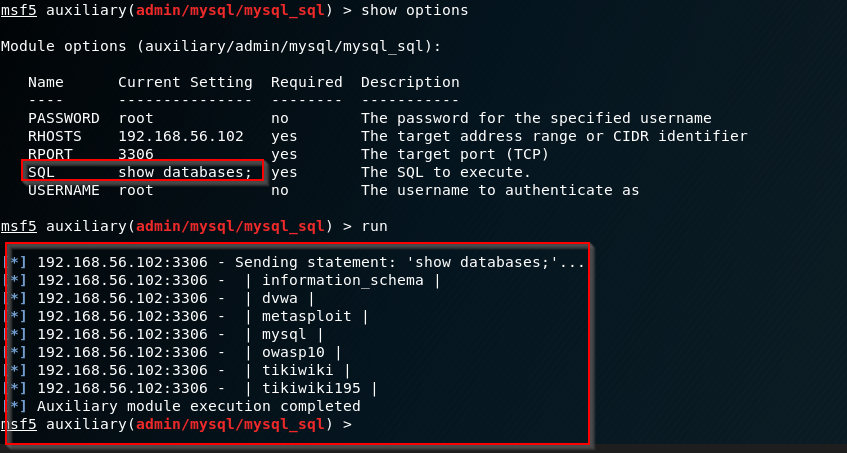
\includegraphics[width=0.98\textwidth,height=0.80\textheight,keepaspectratio]{img/msf_mysql_sql.png}
\end{center}
\end{frame}

\begin{frame}{Ejercicio}
\small
\lead{Realiza un ataque offline al fichero shadow de Metasploitable2}
\begin{columns}[T]
  \begin{column}{0.62\textwidth}
  \begin{itemize}
  \item Para ello, deberás juntar el fichero \cmd{passwd} (usuarios) y el fichero \cmd{shadow} (contraseñas) mediante:
    \begin{itemize}
    \item \cmd{unshadow passwd.txt shadow.txt > passwords}
    \end{itemize}
  \item A partir de ese fichero, ya puedes lanzar John the Ripper
  \end{itemize}
  \end{column}
  \begin{column}{0.36\textwidth}
    \centering
\includegraphics[width=\textwidth,height=0.55\textheight,keepaspectratio]{img/sl038_1.jpg}
  \end{column}
\end{columns}
\end{frame}

\begin{frame}{Ejercicio}
\small
\begin{columns}[T]
  \begin{column}{0.62\textwidth}
  \begin{itemize}
  \item John the Ripper se puede usar también para romper el cifrado de múltiples formatos, por ejemplo de un fichero ZIP
  \item ¿Serías capaz de romper el cifrado del fichero \href{https://pruebasaluuclm-my.sharepoint.com/:u:/g/personal/joseluis_martinez_uclm_es/EUKSZSpi5AdBp-1ojNaeo6MBD3OzsMyW1HX7fclz2MfZgQ?e=wqH52H}{reto1}?
    \begin{itemize}
    \item Pista: usa \cmd{zip2john} para extraer la clave cifrada del fichero y, sobre esa salida, ya puedes lanzar John
    \item \cmd{zip2john reto1.zip > reto1.hash}
    \item \cmd{john -{}-wordlist=rockyou.txt reto1.hash}
    \end{itemize}
  \end{itemize}
  \end{column}
  \begin{column}{0.36\textwidth}
    \centering
\includegraphics[width=\textwidth,height=0.55\textheight,keepaspectratio]{img/sl039_1.jpg}
  \end{column}
\end{columns}
\end{frame}

\begin{frame}{Ejercicio}
\small
\begin{center}
\includegraphics[width=0.78\textwidth,height=0.6\textheight,keepaspectratio]{img/sl040_1.jpg}
\end{center}
  \begin{itemize}
  \item Resuelve la máquina \href{https://app.hackthebox.com/starting-point}{Crocodile} de HackTheBox (Starting Point)
  \end{itemize}
\end{frame}

\section{Captura de credenciales en red: LLMNR/NBT-NS}

\begin{frame}[allowframebreaks]{LLMNR/NBT-NS poisoning attack}
\small
  \begin{itemize}
  \item LLMNR (Link-Local Multicast Name Resolution) y NBT-NS (NetBIOS Name Service) son protocolos usados en redes Windows para resolver nombres de host cuando el DNS falla.
  \item Permiten que los equipos descubran otros dispositivos localmente sin necesidad de un servidor DNS.
  \item ¿En qué consiste el ataque?
    \begin{itemize}

  \item Un atacante se coloca en la red local y escucha las peticiones LLMNR/NBT-NS de los equipos.
  \item Cuando una máquina intenta resolver un nombre no existente (por ejemplo, \texttt{\textbackslash\textbackslash servidor}), el atacante responde falsamente haciéndose pasar por ese servidor.
  \item El equipo víctima envía sus credenciales (hashes NTLMv2) al atacante.
    \end{itemize}
  \item Técnica MITRE ATT\&CK: \href{https://attack.mitre.org/techniques/T1557/001/}{T1557.001 --- LLMNR/NBT-NS Poisoning and SMB Relay}
  \end{itemize}
\end{frame}

\begin{frame}[allowframebreaks]{Herramienta: Responder}
\small
  \begin{itemize}
  \item La herramienta \href{https://github.com/lgandx/Responder}{Responder} suplanta servicios de red comunes (SMB, HTTP, LDAP, etc.) para capturar los hashes NTLMv2:
    \begin{itemize}
    \item \cmd{responder -I eth0 -wv}
    \item Permite después realizar ataques offline (cracking de los hashes capturados)
    \item Y ataques de \emph{relay}, si se combina con herramientas como \href{https://github.com/fortra/impacket}{ntlmrelayx} (Impacket)
    \end{itemize}
  \item Mitigaciones
    \begin{itemize}
    \item Deshabilitar LLMNR y NBT-NS en entornos corporativos.
    \item Implementar DNS fiable y autenticación basada en Kerberos.
    \item Usar SMB signing y seguridad de red avanzada (LAPS, EDR, etc.).
    \end{itemize}
  \end{itemize}
\end{frame}

\begin{frame}{Ejercicio}
\small
\begin{center}
\includegraphics[width=0.78\textwidth,height=0.6\textheight,keepaspectratio]{img/sl043_1.jpg}
\end{center}
  \begin{itemize}
  \item Realiza un ataque usando la herramienta \href{https://github.com/lgandx/Responder}{Responder}. A partir de los hashes capturados, se pueden aplicar ataques offline (John the Ripper) para obtener las credenciales. \href{https://www.youtube.com/watch?v=-k_LXWAhG-c}{Ejemplo}
  \end{itemize}
\end{frame}

\section{Ataques a tokens en la nube}

\begin{frame}{Token Abuse}
\small
\lead{Token Abuse en Azure / Entra ID: tipos de token}
  \begin{itemize}
  \item Las organizaciones modernas autentican en la nube mediante tokens JWT: robar un token equivale a robar las credenciales sin conocer la contraseña.
  \item Tipos de token en Azure / Entra ID:
    \begin{itemize}
    \item \textbf{Access Token:} JWT de corta vida (\textasciitilde{}1\,h). Autoriza el acceso a un recurso concreto (API, Graph\dots{})
    \item \textbf{Refresh Token:} mayor duración. Permite obtener nuevos access tokens sin reautenticación
    \item \textbf{PRT (Primary Refresh Token):} vida larga (\textasciitilde{}90 días), almacenado en el dispositivo unido a Entra ID. Comprometer un PRT equivale a un Golden Ticket en el Active Directory clásico
    \item \textbf{ID Token:} contiene los claims de identidad del usuario (no autoriza, identifica)
    \end{itemize}
  \item Documentación: \href{https://learn.microsoft.com/en-us/entra/identity-platform/access-tokens}{Microsoft Entra --- Access tokens}
  \end{itemize}
\end{frame}

\begin{frame}{Token Abuse}
\small
\lead{Vectores de ataque y técnicas}
  \begin{itemize}
  \item Vectores de ataque:
    \begin{itemize}
    \item Malware en el endpoint que lee tokens del navegador o del proceso LSASS
    \item Phishing de código de dispositivo (Device Code Phishing)
    \item Acceso físico al equipo unido a Entra ID (extracción del PRT vía DPAPI)
    \item Sesiones de navegador no cerradas, o tokens almacenados en disco o en sincronización cloud
    \end{itemize}
  \item Técnicas de abuso de tokens:
    \begin{itemize}
    \item \textbf{Pass-the-Token:} usar un token robado para autenticarse (análogo a Pass-the-Hash)
    \item \textbf{PRT Hijacking:} extraer el PRT para generar nuevos tokens sin MFA
    \item \textbf{Device Code Phishing:} engañar al usuario para que autorice un token vía un código de 8 dígitos
    \item \textbf{Refresh Token Theft:} un refresh token robado genera access tokens indefinidamente
    \item \textbf{Golden SAML:} forjar aserciones SAML con la clave privada robada del IdP
    \end{itemize}
  \item Técnica MITRE ATT\&CK: \href{https://attack.mitre.org/techniques/T1528/}{T1528 --- Steal Application Access Token}
  \end{itemize}
\end{frame}

\begin{frame}{Token Abuse}
\small
\lead{Herramientas y mitigaciones}
  \begin{itemize}
  \item Herramientas:
    \begin{itemize}
    \item \href{https://github.com/Gerenios/AADInternals}{AADInternals} (PowerShell): extraer el PRT, crear tokens y administrar Entra ID
    \item \href{https://github.com/dirkjanm/ROADtools}{roadrecon} (Python): enumerar Azure AD / Graph API
    \item \href{https://github.com/gentilkiwi/mimikatz}{mimikatz}: módulo DPAPI, para extraer el PRT de LSASS en un Windows unido a Entra ID
    \item \href{https://github.com/rvrsh3ll/TokenTactics}{TokenTactics}: manipulación avanzada de tokens de Entra ID
    \end{itemize}
  \item Mitigaciones clave:
    \begin{itemize}
    \item \href{https://learn.microsoft.com/en-us/entra/identity/conditional-access/concept-continuous-access-evaluation}{CAE} (Continuous Access Evaluation): revocación de tokens en tiempo real
    \item Conditional Access, con restricciones de ubicación y de dispositivo
    \item FIDO2 / Passkeys: autenticación sin contraseña ni token robable
    \item Token binding y reducción de la vida útil del refresh token
    \end{itemize}
  \end{itemize}
\end{frame}


\begin{frame}[allowframebreaks]{Resumen}
\begin{center}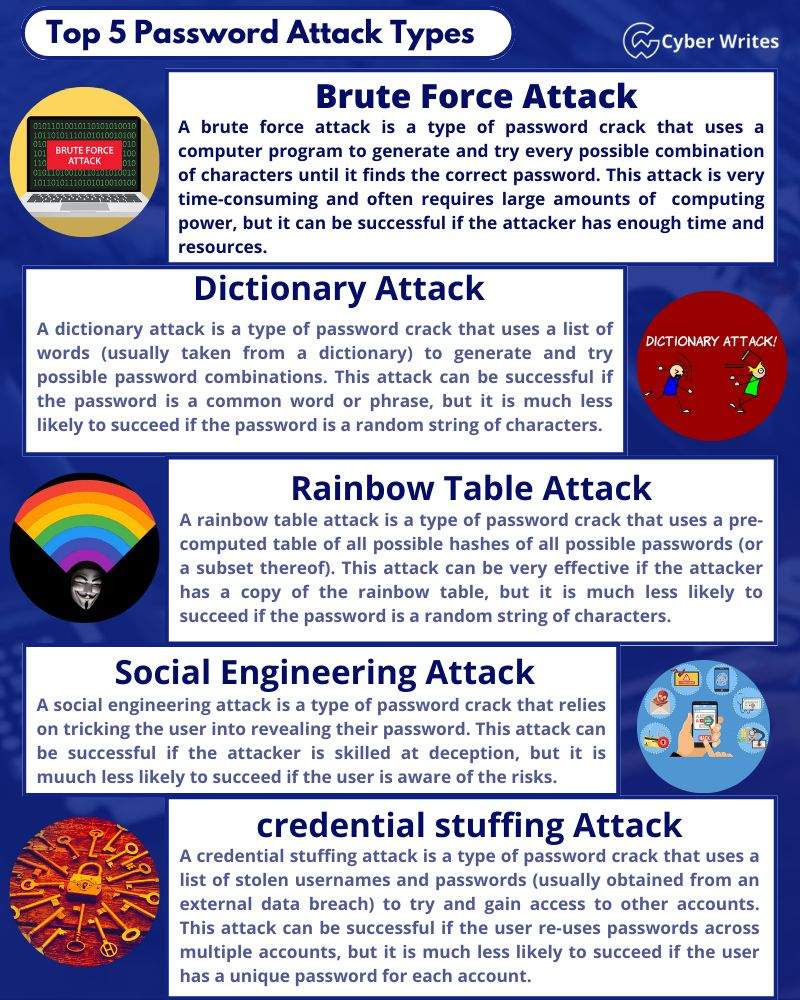
\includegraphics[width=0.78\textwidth,height=0.6\textheight,keepaspectratio]{img/sl045_1.jpg}
\end{center}
\end{frame}

\section{Ejercicios}

\begin{frame}{Ejercicio}
\small
\begin{columns}[T]
  \begin{column}{0.62\textwidth}
  \begin{itemize}
  \item Resuelve el siguiente reto de TryHackMe: \href{https://tryhackme.com/room/crackthehash}{Crack The Hash}
  \item Útil para identificar de qué hash se trata:
    \begin{itemize}
    \item La herramienta \cmd{hash-identifier}
    \item Un cracker online: \href{https://crackstation.net/}{CrackStation}
    \end{itemize}
  \end{itemize}
  \end{column}
  \begin{column}{0.36\textwidth}
    \centering
\includegraphics[width=\textwidth,height=0.55\textheight,keepaspectratio]{img/sl047_1.jpg}
  \end{column}
\end{columns}
\end{frame}

\begin{frame}{Ejercicio}
\small
\begin{columns}[T]
  \begin{column}{0.62\textwidth}
  \begin{itemize}
  \item Resuelve la máquina \href{https://tryhackme.com/room/bruteit}{Brute-It} de TryHackMe, para ello necesitas:
    \begin{itemize}
    \item Enumeration
      \begin{itemize}
      \item Content Discovery
      \end{itemize}
    \item Exploitation
      \begin{itemize}
      \item Login Brute Forcing
      \item John the Ripper sobre un id\_rsa (Hash cracking)
      \end{itemize}
    \end{itemize}
  \end{itemize}
  \end{column}
  \begin{column}{0.36\textwidth}
    \centering
\includegraphics[width=\textwidth,height=0.55\textheight,keepaspectratio]{img/sl048_1.jpg}
  \end{column}
\end{columns}
\end{frame}

\begin{frame}{Ejercicio}
\small
\begin{columns}[T]
  \begin{column}{0.62\textwidth}
  \begin{itemize}
  \item Resuelve la máquina \href{https://tryhackme.com/r/room/brooklynninenine}{Brooklyn-nine-nine} de TryHackMe, para ello:
    \begin{itemize}
    \item Enumeration
      \begin{itemize}
      \item Leak información vía ftp
      \end{itemize}
    \item Exploitation
      \begin{itemize}
      \item Login Brute Forcing
      \end{itemize}
    \end{itemize}
  \end{itemize}
  \end{column}
  \begin{column}{0.36\textwidth}
    \centering
\includegraphics[width=\textwidth,height=0.55\textheight,keepaspectratio]{img/sl049_1.jpg}
  \end{column}
\end{columns}
\end{frame}

\begin{frame}{Ejercicio}
\small
\begin{columns}[T]
  \begin{column}{0.62\textwidth}
  \begin{itemize}
  \item Resuelve la máquina \href{https://tryhackme.com/room/hackernote}{Hackernote} de TryHackMe, para ello necesitas:
    \begin{itemize}
    \item Escaneo + Enumeración
    \item \dots{} y aplicar fuerza bruta explotando una debilidad de timing para obtener el usuario
    \item Hydra para sacar la password
    \end{itemize}
  \end{itemize}
  \end{column}
  \begin{column}{0.36\textwidth}
    \centering
\includegraphics[width=\textwidth,height=0.55\textheight,keepaspectratio]{img/sl050_1.jpg}
  \end{column}
\end{columns}
\end{frame}

\begin{frame}{Ejercicio}
\small
\begin{columns}[T]
  \begin{column}{0.62\textwidth}
  \begin{itemize}
  \item Resuelve la máquina \href{https://tryhackme.com/room/cowboyhacker}{Bounty Hacker} de TryHackMe, para ello necesitas:
    \begin{itemize}
    \item Escaneo + Enumeración
    \item Encontrar un fichero con credenciales en ftp
    \item \dots{} y aplicar fuerza bruta basada en diccionario al servicio ssh
    \end{itemize}
  \end{itemize}
  \end{column}
  \begin{column}{0.36\textwidth}
    \centering
\includegraphics[width=\textwidth,height=0.55\textheight,keepaspectratio]{img/sl051_1.jpg}
  \end{column}
\end{columns}
\end{frame}

\begin{frame}{Ejercicio}
\small
\begin{columns}[T]
  \begin{column}{0.62\textwidth}
  \begin{itemize}
  \item Resuelve la máquina \href{https://tryhackme.com/room/easypeasyctf}{Easy Peasy} de TryHackMe, para ello necesitas:
    \begin{itemize}
    \item Escaneo + Enumeración en el puerto 80
    \item Inspeccionar robots.txt y código fuente web
    \item Decodificar hashes con \href{https://www.dcode.fr/base62-encoding}{dcode.fr/base62-encoding}
    \item Enumerar en el puerto 65524
    \item Decodificar md5 en \href{https://md5hashing.net/hash}{md5hashing.net/hash}
    \item Esteganografía con diccionario
    \item Decodificar binario con \href{https://gchq.github.io/CyberChef/}{CyberChef}
    \end{itemize}
  \end{itemize}
  \end{column}
  \begin{column}{0.36\textwidth}
    \centering
\includegraphics[width=\textwidth,height=0.55\textheight,keepaspectratio]{img/sl052_1.jpg}
  \end{column}
\end{columns}
\end{frame}

\begin{frame}{Ejercicio}
\small
\begin{columns}[T]
  \begin{column}{0.62\textwidth}
  \begin{itemize}
  \item Realiza un ejercicio de fuerza bruta basado en diccionario usando herramientas de enumeración como \href{https://www.kali.org/tools/wfuzz/}{wfuzz} o \href{https://github.com/ffuf/ffuf}{ffuf}
  \item Para ello, puedes construir una petición POST (por ejemplo, con la opción \cmd{-{}-request}) frente a la autenticación de DVWA y usar \cmd{FUZZ} y \cmd{FUZ2Z} para fuzzear usuarios y contraseñas
  \end{itemize}
  \end{column}
  \begin{column}{0.36\textwidth}
    \centering
\includegraphics[width=\textwidth,height=0.55\textheight,keepaspectratio]{img/sl053_1.jpg}
  \end{column}
\end{columns}
\end{frame}

\section{Referencias}

\begin{frame}{Referencias}
\footnotesize
\lead{Estándares y guías de referencia}
  \begin{itemize}
  \item NIST SP 800-63B, \emph{Digital Identity Guidelines: Authentication and Lifecycle Management}. \href{https://pages.nist.gov/800-63-3/sp800-63b.html}{pages.nist.gov}
  \item OWASP, \emph{Authentication Cheat Sheet}. \href{https://cheatsheetseries.owasp.org/cheatsheets/Authentication_Cheat_Sheet.html}{cheatsheetseries.owasp.org}
  \item OWASP, \emph{Password Storage Cheat Sheet}. \href{https://cheatsheetseries.owasp.org/cheatsheets/Password_Storage_Cheat_Sheet.html}{cheatsheetseries.owasp.org}
  \item OWASP, \emph{Credential Stuffing Prevention Cheat Sheet}. \href{https://cheatsheetseries.owasp.org/cheatsheets/Credential_Stuffing_Prevention_Cheat_Sheet.html}{cheatsheetseries.owasp.org}
  \item OWASP, \emph{Web Security Testing Guide} --- sección de autenticación. \href{https://owasp.org/www-project-web-security-testing-guide/}{owasp.org/www-project-web-security-testing-guide}
  \item Biryukov, Dinu, Khovratovich y Josefsson, \emph{Argon2 Memory-Hard Function for Password Hashing}, \href{https://www.rfc-editor.org/rfc/rfc9106.html}{RFC 9106}, 2021
  \end{itemize}
\end{frame}

\begin{frame}{Referencias}
\footnotesize
\lead{Técnicas MITRE ATT\&CK tratadas en el tema}
  \begin{itemize}
  \item \href{https://attack.mitre.org/techniques/T1110/}{T1110 --- Brute Force} (Password Guessing, Password Cracking, Password Spraying, Credential Stuffing)
  \item \href{https://attack.mitre.org/techniques/T1003/}{T1003 --- OS Credential Dumping}
  \item \href{https://attack.mitre.org/techniques/T1056/001/}{T1056.001 --- Input Capture: Keylogging}
  \item \href{https://attack.mitre.org/techniques/T1557/001/}{T1557.001 --- LLMNR/NBT-NS Poisoning and SMB Relay}
  \item \href{https://attack.mitre.org/techniques/T1528/}{T1528 --- Steal Application Access Token}
  \end{itemize}
\medskip
\lead{Documentación de herramientas}
  \begin{itemize}
  \item \href{https://www.openwall.com/john/doc/}{John the Ripper} --- documentación oficial (Openwall)
  \item \href{https://hashcat.net/wiki/}{Hashcat} --- wiki oficial
  \item \href{https://nmap.org/book/nse-usage.html}{Nmap Scripting Engine} --- capítulo del libro de Nmap
  \item \href{https://book.hacktricks.xyz/brute-force}{HackTricks} --- Brute Force
  \item Hitaj, Gasti, Ateniese y Pérez-Cruz, \emph{PassGAN: A Deep Learning Approach for Password Guessing}, ACNS 2019. \href{https://arxiv.org/abs/1709.00440}{arXiv:1709.00440}
  \end{itemize}
\end{frame}

\begin{frame}[plain]
  \begin{center}
    {\Huge\bfseries\color{uznavy} ¡Gracias!}\\[1em]
    {\large Seguridad en Sistemas Informáticos --- Tema 3.1}
  \end{center}
\end{frame}

\pdfinfo{ /Title () /Author () /Subject () /Keywords () /Creator () /Producer () }
\end{document}